\documentclass[12pt]{article}
\usepackage[table]{xcolor}
\usepackage[shortlabels]{enumitem}
\usepackage{tabularx,xltabular}
\usepackage{graphicx}
\usepackage{hyperref}
\usepackage{verbatim}
\usepackage{geometry}
\usepackage{ulem}
\usepackage[official]{eurosym}
\usepackage{tikz}
\usetikzlibrary{arrows,backgrounds,calc,decorations.markings,patterns,3d}
\usepackage{pgfplots}
\pgfplotsset{compat = newest}
\usetikzlibrary{fit}
\newcommand\addvmargin[1]{
\usetikzlibrary{arrows}
\node[fit=(current bounding box),inner ysep=#1,inner xsep=0]{};}
\usepackage{cancel}
\usepackage{fontspec}
\usepackage{array}  
\geometry{a4paper, top=2cm, left=2cm, right=2cm, bottom=2cm, headsep=1cm}
\usepackage{tabu}
\usepackage{pst-node}
\usepackage{colortbl}
\usepackage{array}
\usepackage{german}
\setlength\parindent{0pt}
\newcolumntype{?}{!{\vrule width 1pt}}
\usepackage{makecell}
\renewcommand{\arraystretch}{2.5}
\usepackage{pbox}
\usepackage{amssymb}
\usepackage{amsmath}
\usepackage{booktabs}
\newcolumntype{L}[1]{>{\raggedright\let\newline\\\arraybackslash\hspace{0pt}}m{#1}}
\newcolumntype{C}[1]{>{\centering\let\newline\\\arraybackslash\hspace{0pt}}m{#1}}
\newcolumntype{R}[1]{>{\raggedleft\let\newline\\\arraybackslash\hspace{0pt}}m{#1}}
\begin{document}
\rightline{Datum: 12.06.2023}
\centerline{{\Large Tägliche Übungen}} 
\vspace{1cm}
\noindent \\


\begin{xltabular}{\textwidth}{|C{0.75cm}|X|C{0.75cm}|X|}
\arrayrulecolor{black}\hline
a)&Berechne die Variable $$-13-1\cdot a+4+6\cdot a=11$$
&
b)&Berechne die Variable $$2\cdot b+3+6\cdot b-18=49$$
\\\hline
c)&Berechne die Variable $$-4+6\cdot y+1\cdot y-6=32$$
&
d)&Berechne die Variable $$-10+6\cdot b-2\cdot b-6=32$$
\\\hline
e)&Berechne die Variable $$-4-1+16\cdot y-7\cdot y=58$$
&
f)&Berechne die Variable $$3\cdot y-1\cdot y+1-8=15$$
\\\hline
\end{xltabular}
\vspace{0.5cm}
\newpage
\rightline{Datum: 12.06.2023}
\centerline{{\large Lösungen Tägliche Übungen}} 
\vspace{0.5cm}

\begin{xltabular}{\textwidth}{|C{0.75cm}|X|}
\arrayrulecolor{black}\hline
a)&\begingroup\setlength{\jot}{-0.03cm}
\tikzstyle{background grid}=[draw, black!15,step=.5cm]
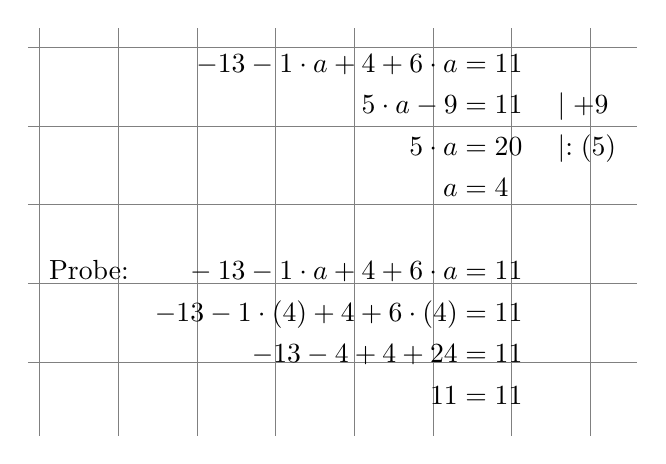
\begin{tikzpicture}[show background grid]
\node[below right] at (0,0.1) {
$\begin{aligned}
-13-1\cdot a+4+6\cdot a &=11& &  \\
5\cdot a - 9 &=11& & \mid + 9\\
5\cdot a &=20& & \mid :\left(5\right)\\
a &=4& & 
\\
\\
\mbox{Probe:}\qquad -13-1\cdot a+4+6\cdot a &=11& &  \\
-13-1\cdot \left(4\right)+4+6\cdot \left(4\right) &=11& &  \\
-13-4+4+24 &=11& &  \\
11 &=11& &  \\
\end{aligned}$};
\end{tikzpicture}
\endgroup
\\\hline
b)&\begingroup\setlength{\jot}{-0.03cm}
\tikzstyle{background grid}=[draw, black!15,step=.5cm]
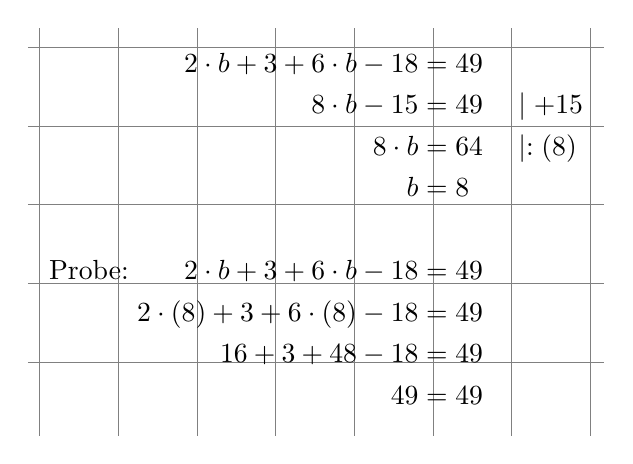
\begin{tikzpicture}[show background grid]
\node[below right] at (0,0.1) {
$\begin{aligned}
2\cdot b+3+6\cdot b-18 &=49& &  \\
8\cdot b - 15 &=49& & \mid + 15\\
8\cdot b &=64& & \mid :\left(8\right)\\
b &=8& & 
\\
\\
\mbox{Probe:}\qquad 2\cdot b+3+6\cdot b-18 &=49& &  \\
2\cdot \left(8\right)+3+6\cdot \left(8\right)-18 &=49& &  \\
16+3+48-18 &=49& &  \\
49 &=49& &  \\
\end{aligned}$};
\end{tikzpicture}
\endgroup
\\\hline
c)&\begingroup\setlength{\jot}{-0.03cm}
\tikzstyle{background grid}=[draw, black!15,step=.5cm]
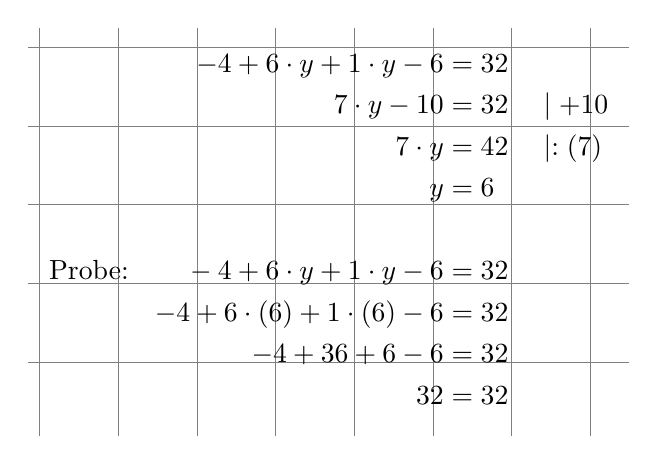
\begin{tikzpicture}[show background grid]
\node[below right] at (0,0.1) {
$\begin{aligned}
-4+6\cdot y+1\cdot y-6 &=32& &  \\
7\cdot y - 10 &=32& & \mid + 10\\
7\cdot y &=42& & \mid :\left(7\right)\\
y &=6& & 
\\
\\
\mbox{Probe:}\qquad -4+6\cdot y+1\cdot y-6 &=32& &  \\
-4+6\cdot \left(6\right)+1\cdot \left(6\right)-6 &=32& &  \\
-4+36+6-6 &=32& &  \\
32 &=32& &  \\
\end{aligned}$};
\end{tikzpicture}
\endgroup
\\\hline
d)&\begingroup\setlength{\jot}{-0.03cm}
\tikzstyle{background grid}=[draw, black!15,step=.5cm]
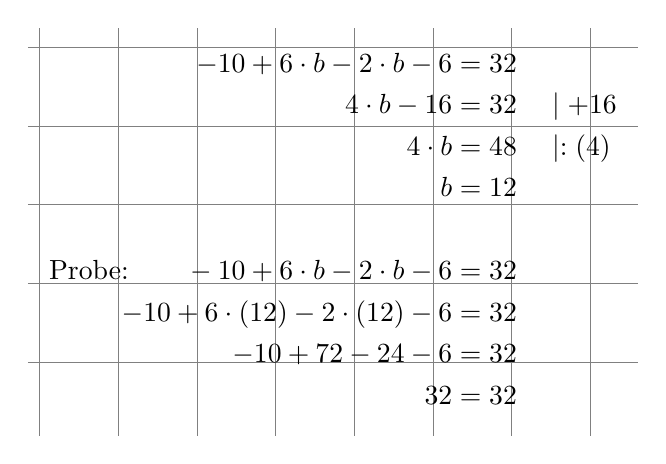
\begin{tikzpicture}[show background grid]
\node[below right] at (0,0.1) {
$\begin{aligned}
-10+6\cdot b-2\cdot b-6 &=32& &  \\
4\cdot b - 16 &=32& & \mid + 16\\
4\cdot b &=48& & \mid :\left(4\right)\\
b &=12& & 
\\
\\
\mbox{Probe:}\qquad -10+6\cdot b-2\cdot b-6 &=32& &  \\
-10+6\cdot \left(12\right)-2\cdot \left(12\right)-6 &=32& &  \\
-10+72-24-6 &=32& &  \\
32 &=32& &  \\
\end{aligned}$};
\end{tikzpicture}
\endgroup
\\\hline
e)&\begingroup\setlength{\jot}{-0.03cm}
\tikzstyle{background grid}=[draw, black!15,step=.5cm]
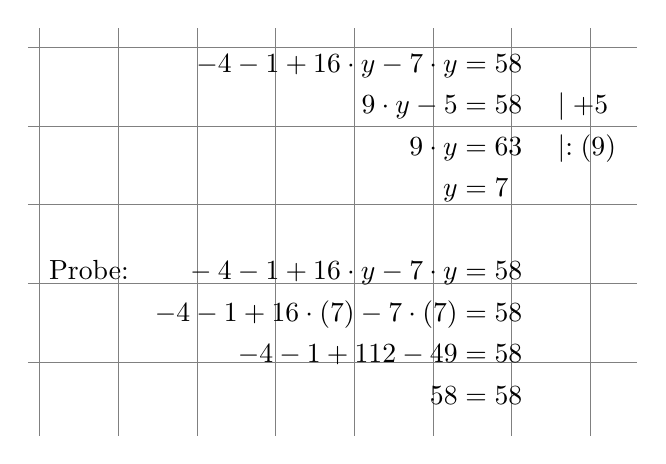
\begin{tikzpicture}[show background grid]
\node[below right] at (0,0.1) {
$\begin{aligned}
-4-1+16\cdot y-7\cdot y &=58& &  \\
9\cdot y - 5 &=58& & \mid + 5\\
9\cdot y &=63& & \mid :\left(9\right)\\
y &=7& & 
\\
\\
\mbox{Probe:}\qquad -4-1+16\cdot y-7\cdot y &=58& &  \\
-4-1+16\cdot \left(7\right)-7\cdot \left(7\right) &=58& &  \\
-4-1+112-49 &=58& &  \\
58 &=58& &  \\
\end{aligned}$};
\end{tikzpicture}
\endgroup
\\\hline
f)&\begingroup\setlength{\jot}{-0.03cm}
\tikzstyle{background grid}=[draw, black!15,step=.5cm]
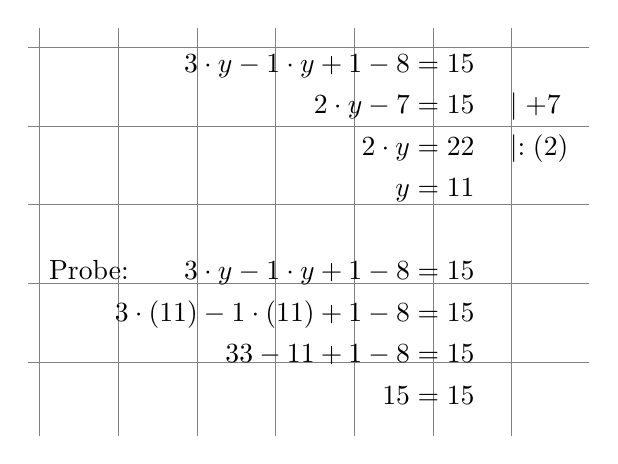
\begin{tikzpicture}[show background grid]
\node[below right] at (0,0.1) {
$\begin{aligned}
3\cdot y-1\cdot y+1-8 &=15& &  \\
2\cdot y - 7 &=15& & \mid + 7\\
2\cdot y &=22& & \mid :\left(2\right)\\
y &=11& & 
\\
\\
\mbox{Probe:}\qquad 3\cdot y-1\cdot y+1-8 &=15& &  \\
3\cdot \left(11\right)-1\cdot \left(11\right)+1-8 &=15& &  \\
33-11+1-8 &=15& &  \\
15 &=15& &  \\
\end{aligned}$};
\end{tikzpicture}
\endgroup
\\\hline
\end{xltabular}
\vspace{0.5cm}
\end{document}